
Before analysing the concept of the virtual network, a few basic concepts of the
graph theory have to be discussed.  The following paragraphs are certainly not
intended as a new contribution to that theory; they merely allow the reader who
is not familiar with this subject to understand the basic concepts on
which the virtual network is founded.  These few pages are based on the
excellent book by Minoux and Bartnik \footnote {Minoux M. and Bartnik G., 1986,
"Graphes, Algorithmes, Logiciels", Dunod informatique.  Interested readers will
certainly like the book by Gondrand M. , Minoux M., 1979, "Graphes et
Algorithmes", Eyrolles.  These two books have been chosen because they deal with
and clearly explain most of the classical algorithms of the graph theory, both
from a methodological viewpoint and from the viewpoint of computer science.  The
complexity of the algorithms presented is systematically calculated, allowing for a
motivated choice between the different algorithms, according to the particular
conditions of the model to be developed.}.




\section{Concepts}

\subsection{Graph}

A graph G = [X, U] is determined by :

\begin{itemize}
\item A set X of which the elements x $\in$ X are called vertices or nodes.
N = \#X  represents the number of nodes. The graph is said to be of the Nth
order.  The nodes are numbered i= 1..N.
\item a set U of which the elements u $\in$ U are ordered couples of nodes,
called arrows. If u = ($x_1,x_2$) is an arrow of G, $x_1$ is the extremity at
the beginning of and $x_2$ the extremity at the end of u. The number of arrows
is indicated by M= \#U.
\end{itemize}




\subsection{Successors and predecessors}


$x_2$ is said to be a successor of $x_1$ if there is an arrow starting at $x_1$
and ending at $x_2$. The set of successors of a node x $\in$ X is indicated by
$\Gamma_x$.

$x_2$ is said to be a predecessor of $x_1$ if there is an arrow ($x_2,x_1$). The
set of predecessors of x $\in$ X can then be indicated by $\Gamma_x^{-1}$.




\subsection{Complete graph}


A graph G = [X,U] is said to be complete if for each pair of nodes ($x_1,x_2$)
there is at least one arrow ($x_1,x_2$) or ($x_2,x_1$).

A transportation network is, therefore, seldom, if ever, a complete graph.




\subsection{Orientation of a graph}


A non ordered pair ($x_1,x_2$), called the link ($x_1,x_2$), is connected to
each arrow ($x_1,x_2$), to the ordered pair ($x_1,x_2$).  A link is thus a non
oriented arrow. A graph G = [X,U] is a non oriented graph if the set U is a set
of links.

A transportation network can be oriented or not.  In an urban network, for
instance, it is important to take one-way traffic into account.  This type of
network is thus oriented.  For large networks for national transportation, on
the other hand, a non oriented graph can be used since each arrow can be
traversed in two directions at the same cost.

However, although the virtual network is to be used on networks of the second type,
it has to be oriented, for reasons that will be explained later.





\subsection{Density of a graph}


The density of a graph is the relationship between the number of arrows (links)
of a graph and the number of arrows (links) of which a complete graph having the
same number of nodes consists. In the case of an oriented graph, the density is
:

$$\frac{M}{N(N-1)} $$

In the case of a non oriented graph, the density is expressed by :

$$\frac{2M}{N(N-1)} $$


A transportation network (as well as the virtual network that can be generated from ) is
therefore a graph with a low density. A node, indeed, is never directly linked
to all the other nodes.  As a general rule, a node is attached to 3 or 4 other
nodes at the most.  This characteristic can influence the choice of the
algorithm that will be used to calculate the pathes.

These few basic concepts being clarified, the notion of multi-modal network
remains to be defined.  The adjective multi-modal covers two separate problems :

\begin{itemize}
\item The choice of the proper transportation mode (road, railway, inland waterways)
\item The choice of the means of transportation (Is it an electric or a diesel-powered train?
Is it a 300 or a 1000 ton ship?)
\end{itemize}

If the only transportation modes considered are the terrestrial ones (trucks,
trains and ships), the multi-modal network is composed of three distinct
mono-modal networks : the road network, the railway network and the network of inland
waterways.  Each network is characterized by one single transportation mode, but
different means of transportation are possible.  The different networks are
interconnected by common terminals and/or ports.

The multi-modal network consists of a set of nodes and a set of links. Each link
represents a trunk that can be used by only one transportation mode, but by different
transportation means.

In the multi-modal network as it has been defined, it is possible to change of
transportation modes and means, and to use several times the same mode or means
of transportation to reach a destination.  Imagine loading the goods into a
lorry, subsequently using waterways, and again transferring the goods into a
lorry to reach the final destination.  The travel route consists thus of a set
of trunks each one used by one transportation mean, and of several
transshipments. For each of those routes it is important to try to minimize the
total cost.





\section{Intuitive approach}


Let us say that R, T and E represent respectively road, railways and waterways.

Firstly, the costs linked to the expenses for loading and transshipping can be
considered as weights to be connected to the nodes of a network whereas the
costs linked to the shipping itself are connected to the links of the
network.

It is, however, necessary to be able to connect a weight to a node in a
conditional way.  The cost of loading or transshipping is only borne if the
goods are indeed loaded or transshipped.  In other words, the transition from
one link to another often takes place without having to change the mode or means
of transportation.

Moreover, the weight of the nodes is almost never the same.  To convince
yourself you need only to observe any loading port along the Canal
Albert/Albertkanaal (Belgium). The canal allows ships of up to 9000 tons but
many of the ships on the canal are more modest ones.  It goes without saying
that, at the same port, the cost of loading a small ship differs from the cost
of loading a large one.

The basic idea of the method and of the algorithm that will be proposed here, is to
create a virtual network, starting from a real network. In this virtual network
a link is created for all the elements to which a weight will be connected.

The solution can first be presented in an intuitive way, by using the example of
a simple waterways network, as shown in figure \ref{f3_1}.


\begin{figure}[htbp]
\centerline{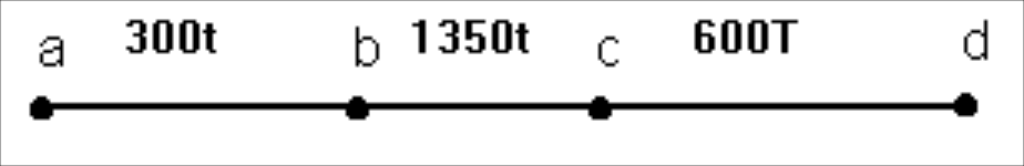
\includegraphics[width=7cm]{f3_1.png}}
\caption{\label{f3_1} Simple network of waterways}
\end{figure}

This network consists of 4 nodes and 3 links.  The links represent waterways
that can support ships of 300, 1350 and 600 tons respectively.

To get from node a to node d, the least expensive route may imply a transshippment
of the goods at node b to a ship of 1000 or 1350 tons, and transferring the goods
to a ship of 600 tons at node c.

Another possibility is to start using ships of 600 tons at node b and keep using
these to get to d.

Finally, an entire trip with ships of 300 tons would also be possible.

Although this network is a very simple one, it clearly reflects the problem of
the modal choice.

The basic idea of the proposed method is to create a virtual network, starting
from a real network.  In the virtual network all the weights, whether linked to
links or to nodes, will be assigned to links.  The notation used for the
identification codes of the nodes in this virtual network, makes it possible to
immediately know the type of cost that has to be connected to each link.  The virtual network derived from the real network presented above is represented in
figure \ref{f3_2}.


\begin{figure}[htbp]
\centerline{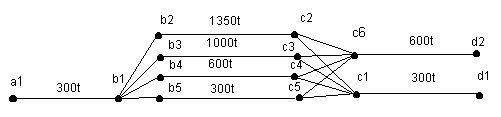
\includegraphics[width=12cm]{f3_2.png}}
\caption{\label{f3_2} Corresponding virtual network}
\end{figure}


The solution implies the creation of a new set of nodes b1-b5, c1-c5, d1-d2 and a new
set of links linking these new nodes.

In a first stage all the existing real links will be split into virtual links
according to the possible means of transportation that can be used :


\begin{itemize}
\item The link (a,b) has not been split because no other ships can pass through a
canal that can only support ships of 300 tons.
\item The link (b,c) has been split into four parts.  A canal of 1350 tons can indeed
accept ships of 300, 600, 1000 and 1350 tons pass through
\item The link (c,d) has been split into two parts, since it is possible to have
ships of 300 and 600 tons pass through the canal.
\end{itemize}


The number of real links has now more than doubled, but they still need to be connected
by means of other virtual links.  These correspond to the transshippment operations.

The real node b, for instance, is represented in the virtual network by four
virtual nodes and by four virtual links.  On these links the costs of
transshippment from a ship of 300 tons to ships of 600, 1000 and 1350 tons can be
assigned.  There is also a virtual link representing the passage from a segment
of 300 tons to another segment of 300 tons.  The weight of that link is zero; it
corresponds to the simple transit of the ship through the (real) node b, without
transshippment operations.

The same mechanism is used for the real node c.  All modal combinations are also
included in the form of virtual links and nodes.  Two links without weight have
been created for ships of 600 and 300 tons 'simple transit'.

In this way, the multi-modal network is represented by a mono-modal network on
which each link has a unique weight representing either the cost of
transportation over a certain distance, either the cost of a possible transshipment.
When a cost is assigned to each link, the cheapest path can be
computed by means of an algorithm such as the algorithm of Johnson.  The
resulting solution is an exact solution, taking all the possible choices into
account and not an heuristic leading to an approximate solution.


\section{Systematic development}

The concept of the virtual network now remains to be developed and the algorithm
for generating a virtual network starting from a real network, must be
written.  In order to make the following pages easier to read, the different
stages of the development of the algorithm will be illustrated by a simple
example of a network.



\subsection{General method}\label{General method}


Given the real network G = [X,U] of figure  \ref{f3_3}. This network is composed
of 4 nodes (\#X = N = 4) a, b, c and d and of 5 links (\#U = M = 5) numbered from 1
to 5.


\begin{figure}[htbp]
\centerline{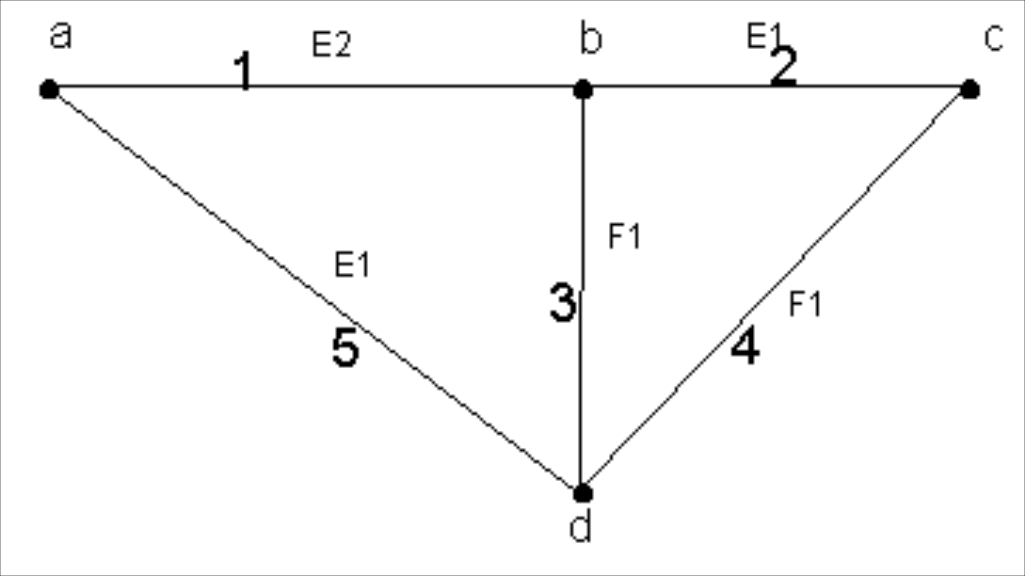
\includegraphics[width=8cm]{f3_3.png}}
\caption{\label{f3_3} Multi-modal network}
\end{figure}

Two modes of transportation are present on the network : the waterways 
\underline{W} and the railways \underline{T}. For the waterways, there are canals (E1
and E2) supporting different sizes of ships, meaning canals of 300 and of 600
tons.  On the links of type E2 it is possible to have ships of the types E1 and
E2.  There is only one type of train, F1 (diesel-powered).  It is important
to use a coherent notation for the means of transportation.  For instance, if a
link supports convoys of type E4, it has to be able to have convoys of the types
E1, E2 and E3.  For this reason the diesel-powered train is indicated by F1
and the electric train by F2, because diesel-powered trains can also
make use of electrified lines, whereas the opposite is impossible.


The table \ref{tab3_1} represents the network :

\begin{table}[htbp]
\begin{center}
\begin{tabular}{cccc}
\hline
Link number & Node 1 & Node 2 & Type of route\\
\hline
1 & a & b & E2\\

2 & b & c & E1\\

3 & b & d & F1\\

4 & d & c & F1\\

5 & a & d & F1\\
\hline
\end{tabular}
\caption{\label{tab3_1} Notation of the real network}
\end{center}
\end{table}


The first stage of the method for creating a virtual network is to examine the
set of links U and to create ($\rightarrow$) for each real link j $\in$ U as
many virtual links $\bar u_j^{tm}$ as there are possible means of transportation
connected to the transportation mode t on that link :

$$\forall _{j\in U} \forall _m u_j \rightarrow \bar u_j^{tm}$$


Each virtual link $\bar u_j^{tm}$ has two virtual end-nodes $\bar x_o^{jtm}$ and
$\bar x_d^{jtm}$ to which an identifier has been assigned, coded in four parts
as follows :


\begin{itemize}

\item  The identification code of the real node i from which the virtual node
is generated,

\item  The identification code of the real link j that has been multiplied (when
several means of transportation are possible on that link),

\item  The identification code of the mode of transportation t on the real link j,

\item  The identification code of the means of transportation m that is possible
on the new virtual link that is generated from the real link j.
\end{itemize}


A virtual node therefore can be identified by $\bar x_i^{jtm}$.

Since each real link has an origin o and a destination d, a real link will
generate the virtual links $\bar u_j^{tm}=(\bar x_o^{jtm},\bar x_o^{jtm})$ (see
table \ref{tab3_2}).


\begin{table}[htbp]
\begin{center}
\begin{tabular}{ccc}
\hline
Real links & Origin of virtual links & Destination of virtual links \\

\hline
1 & a1E2 & b1E2\\

  & a1E1 & b1E1\\

2 & b2E1 & c2E1\\

3 & b3R1 & d3R1\\

4 & d4R1 & c4R1\\

5 & a5E1 & d5E1\\
\hline
\end{tabular}
\caption{\label{tab3_2} Moving links}
\end{center}
\end{table}

\begin{figure}[htbp]
\centerline{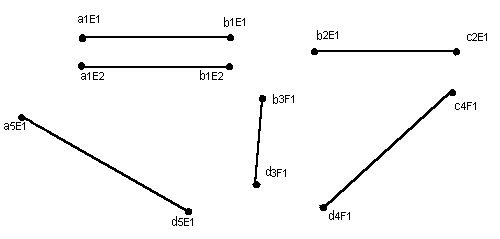
\includegraphics[width=12cm]{f3_4.png}}
\caption{\label{f3_4} Separation of the transport means}
\end{figure}


Starting from this first result (figure \ref{f3_4}), all the links representing
possible transshipments have to be generated.  This operation applies to all
real nodes. In the first phase, all real nodes have been replaced by a set of
virtual nodes.

$$\forall_{i \in X}, X_j \rightarrow \bigcup \bar x_i^{jtm} $$

All virtual nodes referring to the same real node have to be interlinked so as
to represent the set of possible transshipments \footnote {Obviously, it is not
because two links are connected that a transshipment is possible at the connexion.  This case will be discussed later.}. 


$$\forall_k \forall_{k, k\neq l}\rightarrow (\bar x_i^{ktm}, \bar x_i^{lt'm'})$$

For the real node b (figure \ref{f3_5}) this gives the figure \ref{tab3_3} :

\begin{table}[htbp]
\begin{center}
\begin{tabular}{ccc}
\hline
Real node & Origin of virtual links & Destination of virtual links \\

\hline
b & b1E1 & b1E2\\

  & b1E1 & b2E1\\

  & b1E2 & b2E1\\

  & b1E1 & b3R1\\

  & b1E2 & b3R1\\

  & b2E1 & b3R1\\

\hline
\end{tabular}
\caption{\label{tab3_3} Transshipment virtual links}
\end{center}
\end{table}

\begin{figure}[htbp]
\centerline{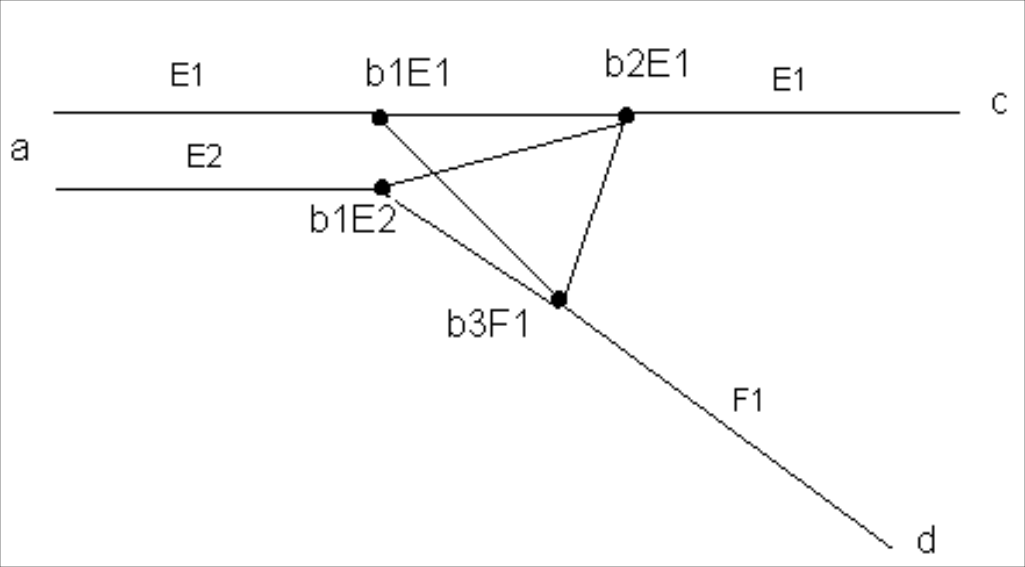
\includegraphics[width=8cm]{f3_5.png}}
\caption{\label{f3_5} Transshipments}
\end{figure}



At this stage there are two types of virtual links :

\begin{itemize}
\item The virtual links representing a distance that has to be covered.
These links represent the links of the real network, possibly multiplied if
there are several possible means of transportation.  Such a link has two virtual
end-nodes originating from two different real nodes.
\item The other virtual links represent all the possible transshipments.
Each virtual node is interlinked with all the other virtual nodes of which the
identification code refers to the same real node, excluding, however, the nodes
generated by the same real link.
\end{itemize}


The last two columns of table \ref{tab3_4} show the costs to be computed on each
virtual link.  In the case of a link that is generated directly from the real
network, it concerns a transfer between two nodes and the weight is a function
of the covered distance.  'Simple transit' costs are represented by a zero in the 'transshipment' column \footnote {In certain cases the cost
is not really zero since this type of links can also serve to represent a cost
linked, for instance, to the passage of a border or to the toll on a motorway.}.
The costs of the type "E2$\rightarrow$E1" represent the costs linked to a
transshipment, in this case the transfer from ships of 600 tons to ships of 300
tons.  There cannot be a cost in the columns "transshipment" and "shipping" at
the same time.


\begin{table}[htbp]
\begin{center}
\begin{tabular}{cccc}
\hline
Origin & Destination & Transshipment cost & Shipping cost\\
\hline
a1E1 & b1E1 & -                   & Cost = $f(distance)$\\

a1E2 & b1E2 & -                   & Cost = $f(distance)$\\

b1E1 & b2E1 & 0 & -\\ 

b1E2 & b1E1 & E2$ \rightarrow$ E1 & -\\

b1E2 & b2E1 & E2$ \rightarrow$ E1 & -\\

b1E1 & b3R1 & E1$ \rightarrow$ R1 & -\\ 

b1E2 & b3R1 & E2$ \rightarrow$ R1 & -

\\b2E1 & b3R1 & E1$ \rightarrow$ R1 & -\\ 

b2E1 & c2E1 & - & Cost = $f(distance)$\\

b3R1 & d3R1 & -                   & Cost = $f(distance)$\\
\hline
\end{tabular}
\caption{\label{tab3_4} Possible operations around the real node b}
\end{center}
\end{table}


If the same operation is repeated for all real nodes, the virtual network looks as the network represented by figure \ref{f3_6}.


\begin{figure}[htbp]
\centerline{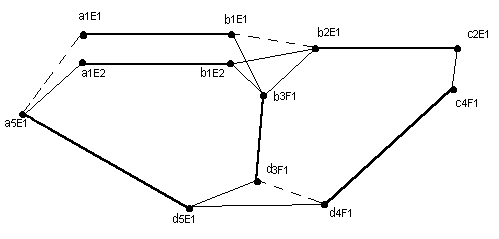
\includegraphics[width=12cm]{f3_6.png}}
\caption{\label{f3_6} Partial virtual network}
\end{figure}

In this network, the boldfaced links represent the links of the real network,
possibly split up.  The links indicated by a dotted line represent the (simple transit( virtual
links.  The transshipments, finally, are indicated by a thin
continuous line.

This method can be transcripted into an algorithm (figure \ref{algo1}), in which the symbol \# is used for the concatenation of the identification code.


\begin{center}
\begin{figure}[htbp]
\center
\fbox{
\begin{minipage}{20cm}
\begin{tabbing}
xxxxx\=xxxxx\=xxxxx\=xxxxx\=xxxxx\=xxxxx\=xxxxx\=xxxxx\=xxxxx\=xxxxx\=\kill
\bf {DEFINE} \\
tab1, tab2: arrays of virtual nodes \\ t1, t2 : indexes in these arrays\\
\\

\bf {BEGIN}\\
t1 $\leftarrow$ 1\\
\bf {FOR} j = 1 $\rightarrow$ mode $\leftarrow$ \it { transport mode on link j}\\
\> k $\leftarrow$ \it {number of transport means on link j}\\
\> \bf {FOR} l = 1 $\rightarrow$ k\\
\> \>  n1 $\leftarrow$\it {start node of link j}\\
\> \> n2 $\leftarrow$\it {end node of link j}\\
\> \> node1 $\leftarrow$ n1\#j\#mode\#k\\
\> \>  node2 $\leftarrow$ n2\#j\#mode\#k\\
\> \>  \it { Save link(node1, node2)}\\
\> \> tab[t1] $\leftarrow$ node1\\
\> \>  tab[t+1] $\leftarrow$ node2\\
\> \> t1 $\leftarrow$ t1 + 2\\
\>  \bf {END FOR} i\\
\bf {END FOR} j\\
\\
\bf {FOR} k = 1 $\rightarrow$ N\\
\> tab2[ ] $\leftarrow$ \it{part of tab1[ ] generated from node k}\\
\> t2 $\leftarrow$ \it {size of tab2[ ]}\\
\> \bf{FOR}  i = 1 $\rightarrow$ t2\\
\> \> \bf{FOR} j = i+1 $\rightarrow$ t2\\
\> \> \> \it{Save link (tab2[i], tab2[j])}\\
\> \> \bf{END FOR} j\\
\> \bf {END FOR} i\\
\bf {END FOR} k\\
\bf {END}\\
\end{tabbing}
\end{minipage}
}
\caption{\label{algo1} Basic algorithm}
\end{figure}
\end{center}




\subsection{The entry-nodes}


One problem remains unsolved : although it is possible to travel within the
virtual network, it is not possible to enter it or to leave it !  The final
user wants to find a travel route between the real nodes a and b and not between
the virtual nodes axxx and bxxx.  Moreover, there is a cost linked to entering
and leaving the network since the goods have to be loaded and unloaded.

The virtual links and nodes again offer a solution.  In the example of node b,
for instance, it is sufficient to create a new virtual node b000 and to link it
to all other virtual nodes generated for that real node.  All the new links
represent the costs of loading and unloading the goods.


$$x_i \rightarrow \bar x_i^{000}$$

$$\forall_i \forall_{ktm} \rightarrow (\bar x_i^{ktm}, \bar x_i^{000})$$



This lead, for the node b, to table \ref{tab3_5} and figure \ref{f3_7}:


\begin{figure}[htbp]
\centerline{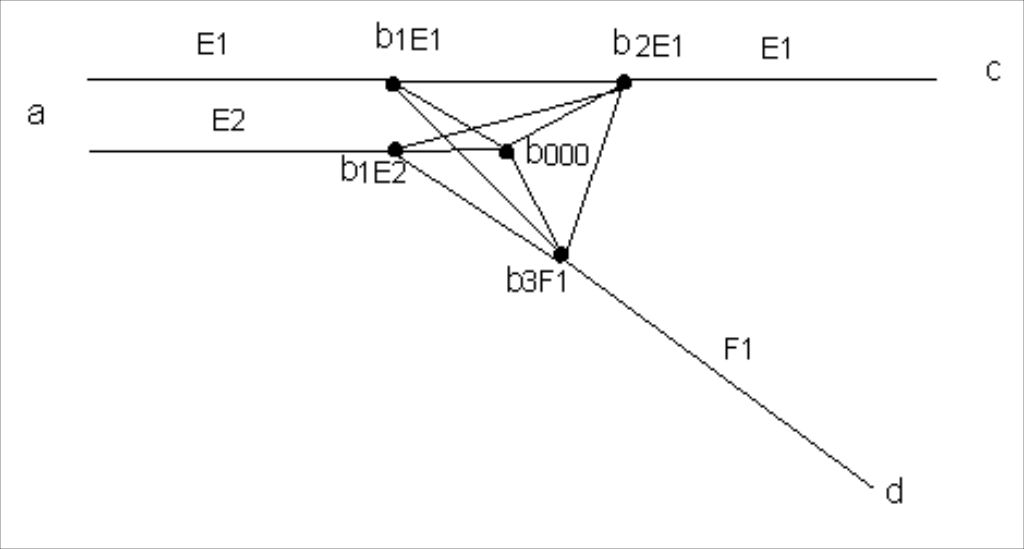
\includegraphics[width=12cm]{f3_7.png}}
\caption{\label{f3_7} Loadings/Unloadings in a virtual network}
\end{figure}

\begin{table}[htbp]
\begin{center}
\begin{tabular}{ccc}
\hline
Origin & Destination & Cost\\
\hline
b000 & b1E1 & 0 $\rightarrow$ E1\\

b000 & b1E2 & 0 $\rightarrow$ E2\\

b000 & b2E1 & 0 $\rightarrow$ E1\\

b000 & b3R1 & 0 $\rightarrow$ R1\\
\hline
\end{tabular}
\caption{\label{tab3_5} Costs on (un)loading virtual links}
\end{center}
\end{table}

In table \ref{tab3_5}, the cost represents the initial loading of the goods or their final unloading.

The algorithm shown above has to be modified to take these new virtual
nodes and links into account (see figure \ref{algo2}).


\begin{center}
\begin{figure}[htbp]
\center
\fbox{
\begin{minipage}{20cm}
\begin{tabbing}
xxxxx\=xxxxx\=xxxxx\=xxxxx\=xxxxx\=xxxxx\=xxxxx\=xxxxx\=xxxxx\=xxxxx\=\kill
\bf {DEFINE} \\
tab1, tab2: arrays of virtual nodes \\ t1, t2: indexes in these arrays\\
\\

\bf {BEGIN}\\
t1 $\leftarrow$ 1\\
\bf {FOR} j = 1 $\rightarrow$ mode $\leftarrow$ \it{transport mode on link j}\\
\> k $\leftarrow$ \it {number of transport means on link j}\\
\> \bf {FOR} l = 1 $\rightarrow$ k\\
\> \>  n1 $\leftarrow$\it {start node of link j}\\
\> \> n2 $\leftarrow$\it {end node of link j}\\
\> \> node1 $\leftarrow$ n1\#j\#mode\#k\\
\> \>  node2 $\leftarrow$ n2\#j\#mode\#k\\
\> \>  \it { Save link(node1, node2)}\\
\> \> tab[t1] $\leftarrow$ node1\\
\> \>  tab[t+1] $\leftarrow$ node2\\
\> \> t1 $\leftarrow$ t1 + 2\\
\>  \bf {END FOR} i\\
\bf {END FOR} j\\
\\
\bf {FOR} k = 1 $\rightarrow$ N\\
\> tab2[ ] $\leftarrow$ \it{part of tab1[ ] generated from node k}\\
\> t2 $\leftarrow$ \it {size of tab2[ ]}\\
\> \bf{FOR}  i = 1 $\rightarrow$ t2\\
\> \> \bf{FOR} j = i+1 $\rightarrow$ t2\\
\> \> \> \it{Save link(tab2[i], tab2[j])}\\
\> \> \bf{END FOR} j\\
\> \bf {END FOR} i\\
\\
\> \bf{FOR} i = 1 $\rightarrow$ t2\\
\> \> node $\leftarrow$ \it{"node" part of tab2[i]\#000}\\
\> \> \it{Save link(node, tab2[i])}\\
\> \bf{END FOR} i\\
\bf {END FOR} k\\
\bf {END}\\
\end{tabbing}
\end{minipage}
}
\caption{\label{algo2} Introduction of the (un)loading, virtual links}
\end{figure}
\end{center}




\subsection{The simple transit nodes}

At this stage, it is difficult to apply this method to a real network, as it often contains a serie of nodes that do not represent points where goods
are being loaded/unloaded.  The road network is characterized by a multitude of
crossroads that are also nodes, but where no goods are being loaded.  In the
same way the railway network contains some stations that are
exclusively reserved for the passengers and where transshipments of goods are
impossible.

For these nodes, no transshipment virtual links have to be
generated.

In the example of figure \ref{f3_8}, node b represents an intersection of a
waterway of 600 tons (E2) and another of 300 tons (E1).

\begin{figure}[htbp]
\centerline{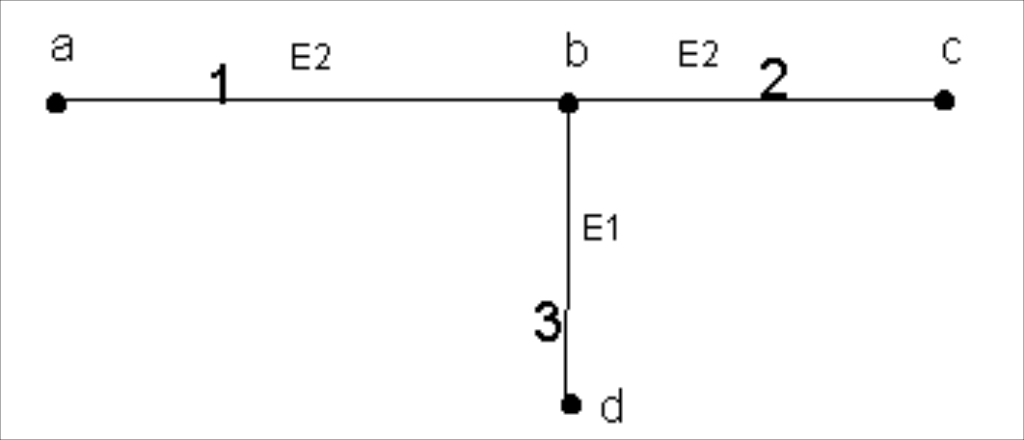
\includegraphics[width=8cm]{f3_8.png}}
\caption{\label{f3_8} Intersection of two waterways}
\end{figure}

The trunks of type E2 also support convoys of type E1.  A ship of 600 tons coming
from segment 1 can therefore continue to segment 2, but not to segment 3.

The previously explained method leads thus to the creation of the virtual nodes listed in table \ref{tab3_6}) :


\begin{table}
\begin{center}
\begin{tabular}{ccccc}
\hline
Real node & Real link & Mode & Means & Virtual node\\
\hline
b & 1 & W & 1 & b1E1\\

b & 1 & W & 2 & b1E2\\

b & 2 & W & 1 & b2E1\\

b & 2 & W & 2 & b2E2\\

b & 3 & W & 1 & b3E1\\
\hline
\end{tabular}
\caption{\label{tab3_6} Simple transit nodes}
\end{center}
\end{table}



The virtual links now need to be generated.  Again, shipping and transshipment virtual links must be generated.  This time, however, only the nodes
referring to the same combination mode-means of transportation (t = t' and m =
m') may be interlinked.  For this reason b1E2 and B2E2 will be interlinked, but
not b1E2 and b3E1 (this last combination would suggest a transshipment from a
ship of 600 tons to a ship of 300 tons and vice versa).  In other words, only
the "simple transit"virtual links are created.  Moreover, since these "transit"
nodes are not points where the network can be entered or left, the b000 node
does not need to be created, nor do the virtual links that are generated from it.


\begin{center}
If (i =  transshipment) or (t = t' and m = m') $\rightarrow
\forall_k \forall_{l} \rightarrow(\bar x_i^{ktm},
\bar x_i^{lt'm'})$\\
If i is a transshipment node $\rightarrow \forall_i
\forall_{ktm}
\rightarrow (\bar x_i^{ktm}, \bar x_i^{000})$
\end{center}

That leads to the creation of the set of links reported in table \ref{tab3_7}
(see also figure \ref{f3_9}).


\begin{table}[htbp]
\begin{center}
\begin{tabular}{cccc}
\hline

Origin & Destination & Transshipment cost & Shipping cost\\
\hline
a1E1 & b1E1 & - & $f(distance)$\\

a1E2 & b1E2 & - & $f(distance)$\\

b2E1 & c2E1 & - & $f(distance)$\\

b2E2 & c2E2 & - & $f(distance)$\\

b3E1 & d3E1 & - & $f(distance)$\\

b1E1 & b2E1 & 0 & -\\

b1E1 & b3E1 & 0 & -\\

b2E1 & b3E1 & 0 & -\\

b1E2 & b3E2 & 0 & -\\
\hline
\end{tabular}
\caption{\label{tab3_7} Virtual network at the intersection}
\end{center}
\end{table}

\begin{figure}[htbp]
\centerline{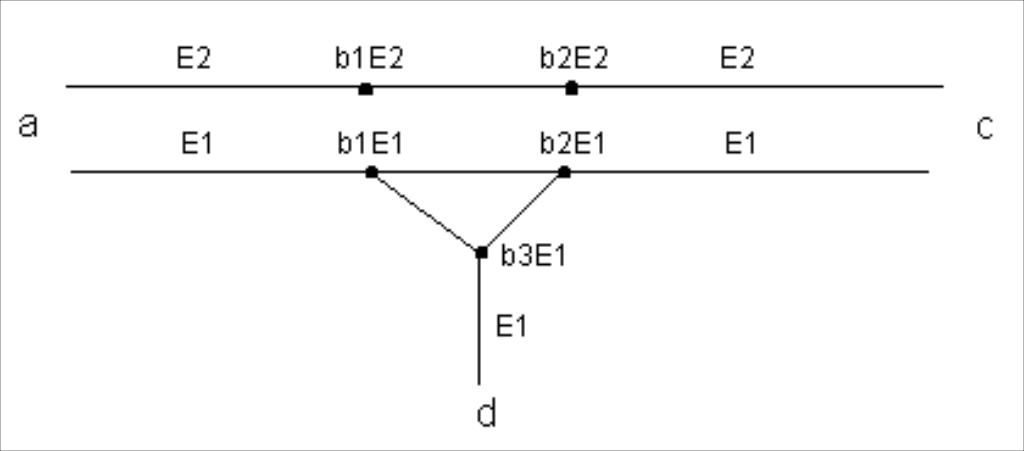
\includegraphics[width=10cm]{f3_9.png}}
\caption{\label{f3_9}  Virtual network at the intersection}
\end{figure}


The method differs according to whether the node is a place where goods are
loaded/unloaded/transshipped or simply a place of transit.  The nodes of the
graph therefore have to be marked as belonging to one of those two categories.

This differentiated treatment (see figure \ref{algo3}) has a very interesting
effect. Indeed, since the "transit" nodes generate less virtual links, the
virtual network itself will consist of clearly less links than the network
generated by the basic algorithm, an effect which will accelerate the processing
time.


\begin{center}
\begin{figure}[htbp]
\center
\fbox{
\begin{minipage}{20cm}
\begin{tabbing}
xxxxx\=xxxxx\=xxxxx\=xxxxx\=xxxxx\=xxxxx\=xxxxx\=xxxxx\=xxxxx\=xxxxx\=\kill
\bf {DEFINE} \\
tab1, tab2: arrays of virtual nodes \\ t1, t2: indexes in these arrays\\
\\

\bf {BEGIN}\\
t1 $\leftarrow$ 1\\
\bf {FOR} j = 1 $\rightarrow$ mode $\leftarrow$ \it{transport mode on link j}\\
\> k $\leftarrow$ \it {number of transport means on link j}\\
\> \bf {FOR} l = 1 $\rightarrow$ k\\
\> \>  n1 $\leftarrow$\it {start node of link j}\\
\> \> n2 $\leftarrow$\it {end node of link j}\\
\> \> node1 $\leftarrow$ n1\#j\#mode\#k\\
\> \>  node2 $\leftarrow$ n2\#j\#mode\#k\\
\> \>  \it {Save link(node1, node2)}\\
\> \> tab[t1] $\leftarrow$ node1\\
\> \>  tab[t+1] $\leftarrow$ node2\\
\> \> t1 $\leftarrow$ t1 + 2\\
\>  \bf {END FOR} i\\
\bf {END FOR} j\\
\\
\bf {FOR} k = 1 $\rightarrow$ N\\
\> tab2[ ] $\leftarrow$ \it{part of tab1[ ] generated from node k}\\
\> t2 $\leftarrow$ \it {size of tab2[ ]}\\
\> \bf{FOR}  i = 1 $\rightarrow$ t2\\
\> \> \bf{FOR} j = i+1 $\rightarrow$ t2\\
\> \> \> \bf{IF} \it{not a transshipment node}\\
\> \> \> \> \bf{AND} \it{"mode" part of tab2[i] = "mode" part of tab2[j]}\\
\> \> \> \> \bf{AND} \it{"means" part of tab2[i] = "means" part of tab2[j])}\\
\> \> \> \bf{OR} \it{transshipment node}\\
\> \> \> \> \> \bf{THEN} \it {Save link(tab2[i], tab2[j])}\\
\> \> \> \bf{END IF}\\
\> \> \bf{END FOR} j\\
\> \bf{END FOR} i\\
\\
\> \bf{FOR} i = 1 $\rightarrow$ t2\\
\> \> \bf{IF} \it{transshipment node} \bf{THEN}\\
\> \> \> node $\leftarrow$ \it{''node'' part of tab2[i]\#000}\\
\> \> \> \it{Save link(node, tab2[i])}\\
\> \> \bf{END IF}\\
\> \bf{END FOR} i\\
\bf {END FOR} k\\
\bf {END}\\
\end{tabbing}
\end{minipage}
}
\caption{\label{algo3} Introduction of the "simples transit virtual links"}
\end{figure}
\end{center}



\subsection{Orientation of the virtual network}


The method hereby proposed leads to the generation of a non oriented virtual
network.  Since each link has to be balanced by a unique weight (a cost), the
use of a non oriented graph creates the problem of the equivalence of weights
when there are transfers from origin to destination or from destination to
origin.

Such an equivalence is to strong hypothesis to be applied to a freight transportation network.  Certain
costs are a function of the direction on the link.  This is, for instance, the
case for loadings and unloadings : experience shows that it often
takes more time to unload than to load a vehicle.

In practice, the algorithm of the virtual network will generate oriented links,
which makes it possible to assign different costs according to the direction of
the virtual link. In order to generate only one (oriented) arrow between two virtual nodes (to avoid unwanted turns during the cheapest path calculation), all the nodes are ``doubled'' by giving them a positive and a negative sign. 

Using the notation used in section \ref{General method}, the virtual network generated around node b and illustrated by figure \ref{f3_7} can be represented as in figure \ref{f3_7b}.

\begin{figure}[htbp]
\centerline{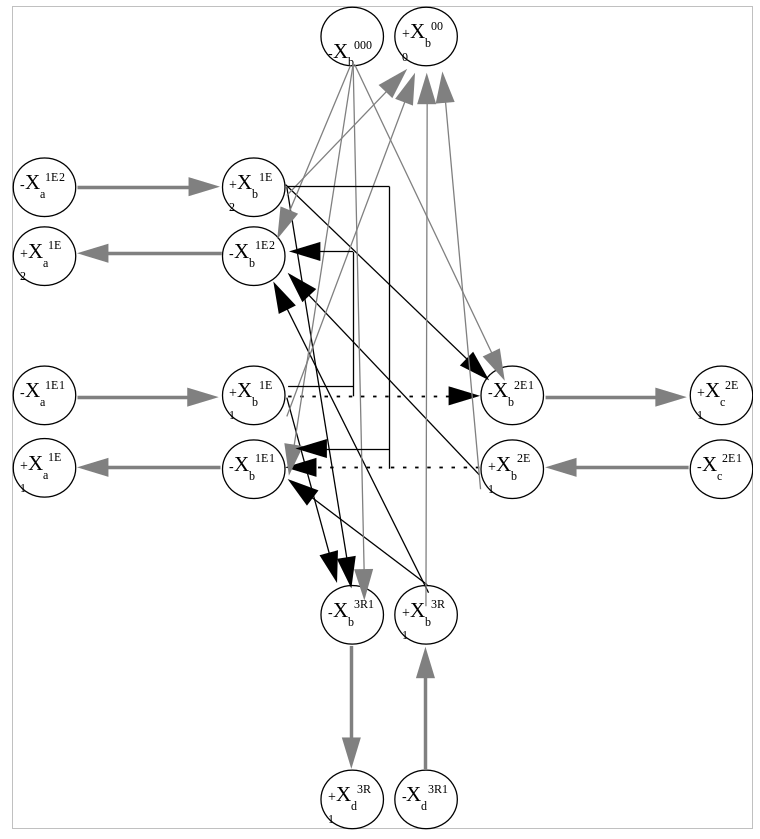
\includegraphics[width=10cm]{f3_7b.png}}
\caption{\label{f3_7b} Oriented virtual network}
\end{figure}


\subsection{Additional control on the generation of the virtual network}


The virtual network, as it has been defined for the moment, is the result of an
automatic procedure.  This way of proceeding, however, implies certain
restrictions, because some transshipment possibilities are generated
automatically whereas these movements are not possible on the real network.
This is, for instance, the case with private ports on inland waterways.  A
particular company may be authorised to load and unload goods there, but this
port does not serve as a public place of transshipment.  Therefore it is
important to be able to control the generation of the virtual network.

This check becomes possible if exclusions lists are kept for the different
nodes of the real network.  In practice it must be possible to define, for each
node of the network, the list of handling operations which would be generated
automatically but which are not possible in reality because of the physical
characteristics of the network at that location.  The generation procedure of
the virtual network is consequently adjusted, since it consults these lists of
exclusions to know whether or not a virtual link can be created.

The final algorithm is is presented in figure \ref{algo4}.

\begin{center}
\begin{figure}[htbp]
\center
\fbox{
\begin{minipage}{20cm}
\begin{tabbing}
xxxxx\=xxxxx\=xxxxx\=xxxxx\=xxxxx\=xxxxx\=xxxxx\=xxxxx\=xxxxx\=xxxxx\=\kill
\bf {DEFINE} \\
tab1, tab2: arrays of virtual nodes \\ t1, t2: indexes in these arrays\\
\\

\bf {BEGIN}\\
t1 $\leftarrow$ 1\\
\bf {FOR} j = 1 $\rightarrow$ mode $\leftarrow$ \it{transport mode on link j}\\
\> k $\leftarrow$ \it {number of transport means on link j}\\
\> \bf {FOR} l = 1 $\rightarrow$ k\\
\> \>  n1 $\leftarrow$\it {start of link j}\\
\> \> node1 $\leftarrow$ +\#n1\#j\#mode\#k and node2 $\leftarrow$ -\#n2\#j\#mode\#k\\
\> \>  \it {Save link(node1, node2)}\\
\> \> tab[t1] $\leftarrow$ node1; tab[t+1] $\leftarrow$ node2\\
\> \> t1 $\leftarrow$ t1 + 2\\
\> \> node1 $\leftarrow$ -\#n1\#j\#mode\#k and node2 $\leftarrow$ +\#n2\#j\#mode\#k\\
\> \>  \it {Save link(node2, node1)}\\
\> \> tab[t1] $\leftarrow$ node1; tab[t+1] $\leftarrow$ node2\\
\> \> t1 $\leftarrow$ t1 + 2\\
\>  \bf {END FOR} i\\
\bf {END FOR} j\\
\\
\bf {FOR} k = 1 $\rightarrow$ N\\
\> tab2[ ] $\leftarrow$ \it{ part of tab1[ ] generated from node k}\\
\> t2 $\leftarrow$ \it {size of tab2[ ]}\\
\> \bf{FOR}  i = 1 $\rightarrow$ t2\\
\> \> \bf {FOR} j = i+1 $\rightarrow$ t2\\
\> \> \> \bf{IF} \it{not a transshipment node}\\
\> \> \> \> \bf{AND} \it{"mode" part of tab2[i] = "mode" part of tab2[j]}\\
\> \> \> \> \bf{AND} \it{"means" part of tab2[i] = "means" part of tab2[j]}\\
\> \> \> \bf{OR} \it{transshipment node}\\
\> \> \> \> \> \bf{THEN IF} \it {non excluded transfer}\\
\> \> \> \> \> \> \bf{IF} \it{``node'' part of tab2[i] > 0}\\ 
\> \> \> \> \> \> \> \bf{THEN} {Save link(tab2[i], tab2[j])}\\
\> \> \> \> \> \> \> \bf{ELSE} {Save link(tab2[j], tab2[i])}\\
\> \> \> \> \> \> \bf{END IF}\\
\> \> \> \bf{END IF}\\
\> \> \bf{END FOR} j\\
\> \bf {END FOR} i\\
\\
\> \bf{FOR} i = 1 $\rightarrow$ t2\\
\> \> \bf{IF} \it{transshipment node} \bf{AND} \it{non excluded transfer} \bf{THEN}\\
\> \> \> node $\leftarrow$ -\#\it{"node" part of tab2[i]\#000}; \it{Save link(node, tab2[i])}\\
\> \> \> node $\leftarrow$ +\#\it{"node" part of tab2[i]\#000}; \it{Save link(tab2[i], node)}\\
\> \> \bf{END IF}\\
\> \bf{END FOR} i\\
\bf {END FOR} k\\
\bf {END}
\end{tabbing}
\end{minipage}
.}
\caption{\label{algo4} Algorithm of generation of a virtual network}
\end{figure}
\end{center}




\section{Assignment of the costs on the virtual links}


The virtual network makes use of four types of distinct costs : loading/unloading,
transshipping, moving and simple transit.  The type of cost to be assigned to
each virtual link can be automatically deducted from the notation used for the
two virtual end-nodes of the link.

For readability reasons, the notation used up to here has been a
notation of the type "b1E1".  It is clear that this type of notation cannot be
used in practice.  NODUS will therefore use a 10 digits integer to represent
the number of the real node, another 10 digits integer for the number of the
real link,  two digits to represent the transportation mode and two digits to
refer to the means of transportation.

As mentioned above, the virtual node is indicated in the following way (see also
table \ref{tab3_8}) :


\begin{enumerate}
\item \underline{Moving (\textbf{``mv''})}: the numbers of the real nodes are different in the two virtual nodes codes (case 1). Always from a - to a + sign.
\item \underline{Simple transit (\textbf{``tr''})}: the number of the real links vary whereas the mode and
the means of transportation have remained the same (case 2). Always from a + to a - sign.
\item \underline{Transshipment (\textbf{``tp''})}: the mode and/or means of transportation vary (case 3). Always from a + to a - sign.
\item \underline{Loading (\textbf{``ld''})/unloading (\textbf{``ul''})}: one of the two real links is "0"
(cases 4a and 4b). Always from a - to a - sign for loading and from a + to a + sign for unloading.
\end{enumerate}



\begin{table}[htbp]
\begin{center}
\begin{tabular}{crcccrccc}
\hline

Case & Node1 & Link1 & Mode1 & Means1 & Node2 & Link2 & Mode2 & Means2\\
\hline
1 & -1000 & 1000 & 1 & 1 & +1001 & 1000 & 1 & 1\\

2 & +1000 & 1000 & 1 & 1 & -1000 & 1001 & 1 & 1\\

3 & +1000 & 1000 & 1 & 1 & -1000 & 1001 & 1 & 2\\

$4_a$ & -1000 & 0 & 0 & 0 & -1000 & 1001 & 1 & 1\\

$4_b$ & +1000 & 1001 & 1 & 1 & +1000 & 0 & 0 & 0\\
\hline
\end{tabular}
\caption{\label{tab3_8} Codification of the virtual links in NODUS}
\end{center}
\end{table}


Different costs correspond to these different cases.  In the following
chapter, a general methodological framework will be provided for the development
of specific cost functions for each application.




\section{Concluding comments}


The virtual network (and NODUS, the software that implements it can be presented as :


\begin{itemize}
\item An exhaustive representation of all possible movements and operations on a
multi-modal transportation network.
\item A systematic way to generate of the elements composing the network
through an automatic procedure.
\item A general representation of a network, adapted to the realisation of a wide
range of different applications.
\item A systematic and codified notation of the elements of the network, allowing to
know the nature of the costs to be assigned to the different links.  This same
notation, based on numbers of virtual nodes coded in four parts, contains all
the necessary information on the modes and means of transportation used.  This
information can be used,  after an assignment on the network, to retrace
the modes and means of transportation that have effectively been used on the
different links composing the route.  This is an important characteristic and a valuable
aspect of the concept of the virtual network.
\end{itemize}


